The CMS detector was designed with two primary physics goals in mind.
First, to study the properties of the Higgs boson; in particular, the nature of electroweak symmetry breaking for which the Higgs mechanism is responsible\footnote{Note that during the design of the CMS detector, the Higgs boson was theorized to exist but had not yet been discovered.}.
Second, to reveal signs of physics beyond the Standard Model which might be present at the TeV scale.
This section discusses technical design aspects of the CMS detector and how they support the physics goals of the CMS experiment.
\subsection{General Design Concepts} \label{sec:cms_overview}
The CMS detector is over 20m in length and nearly 15m in diameter -- it is ``compact'' only in the context of the tremendous size of a detector needed to facilitate the physics goals for which it was designed.
The various components of the CMS detector are shown in Fig.~\ref{fig:cms_schematic}, with humans shown to illustrate the scale (banana not available).

\begin{figure} [htbp!]
    \centering
    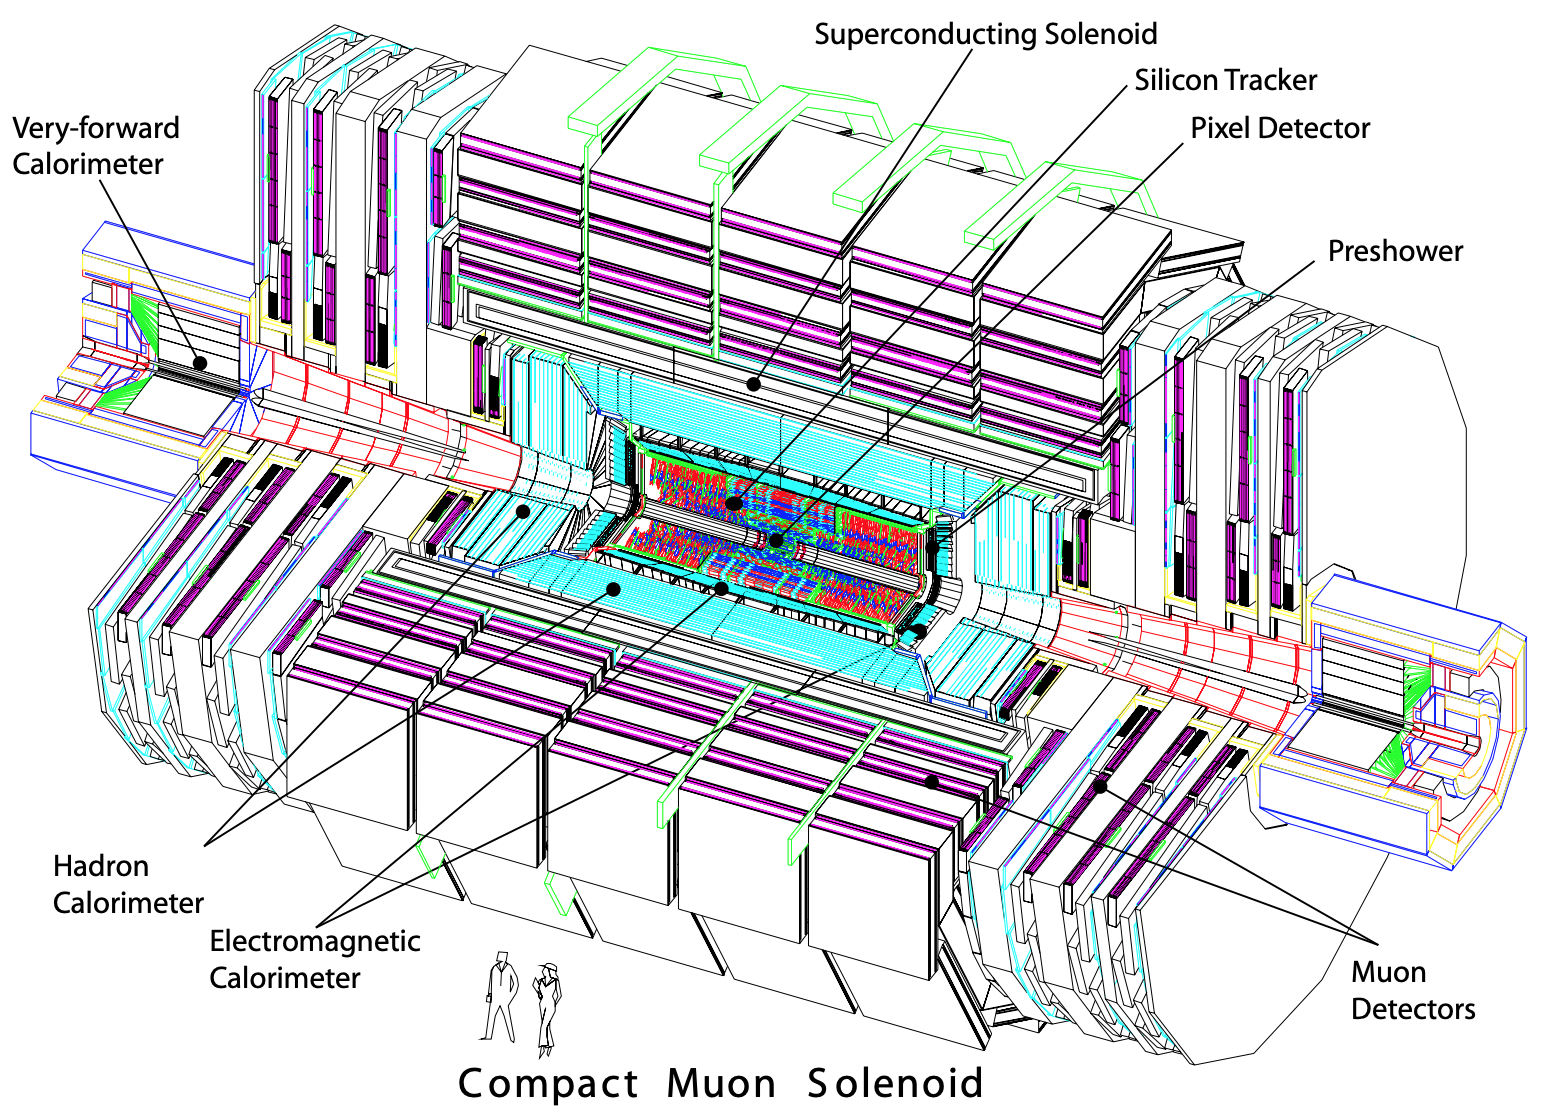
\includegraphics[width=0.8\linewidth]{figures/cms/cms_detector_schematic.png}
    \caption{Schematic of the various components of the CMS detector. Taken from~\cite{Chatrchyan:2008aa}.}
    \label{fig:cms_schematic}
\end{figure}

As its name suggests, the primary feature of the CMS detector is a superconducting solenoid providing a magnetic field of 4~T.
The purpose of the magnetic field is to bend the path of charged particles originating from inelastic proton-proton interactions: the precise spatial resolution of the tracker and muon system allows one to determine a particle's radius of curvature, in turn allowing one to determine the particle's momentum.
Excellent momentum resolution of charged particles supports nearly every physics analysis performed with the CMS detector, but is especialy important for determining the invariant mass of heavy resonances (e.g. studying the properties of the Higgs boson in the H $\to$ ZZ$^{*} \to 4l$ channel), distinguishing between hadronic jets which originate from b quarks from those which originate from gluons or light-flavor quarks (e.g. the H $\to$ bb decay channel and searches for new physics involving final states with b-jets), and for precise resolution of the missing transverse energy (e.g. final states with neutrinos or searches for new physics involving final states with undetected dark matter or supersymmetry candidate particles).

The other major components of the detector include: 
\begin{itemize}
    \item The tracker, which allows for identification and excellent momentum resolution of charged particles.
    \item The electromagnetic calorimeter (ECAL), which allows for identification of electrons and photons, particularly important for H $\to \gamma \gamma$ physics.
    \item The hadronic calorimeter (HCAL), which assists in the identification and momentum resolution of charged hadrons and provides the only handle on measuring neutral hadrons.
    \item The muon system, which enables better momentum resolution of very high energy ($\mathcal O$(TeV)) muons (while the tracker excels in providing good momentum resolution for lower energy, $\mathcal O$(GeV) muons).
\end{itemize}
Each of these components is described in greater detail in the following subsections.

A design consideration common to multiple subdetector components is the goal of hermeticity: a fully hermetic detector is able to measure particles emerging in any direction from an inelatic collision.
In other words, a hermetic detector has full coverage of the $4\pi$ steradians of solid angle surrounding the interaction point.
The CMS detector is not fully hermetic, as it is practically impossible to measure particles which emerge parallel to the LHC's proton beams.
Still, the CMS detector is able to measure very forward particles (with ``forward'' meaning ``close to parallel with the beam axis''), aiding the nearly complete reconstruction of the final state of a given pp interaction, which is essential for resolution of the missing transverse energy.

To expand upon the concepts of hermeticity and the identification of forward particles, we must first introduce the coordinate system used to describe the CMS detector.
Given the cylindrical shape of the detector, standard cylincdrical coordinates form the basis of the coordinate system: the $\hat{z}$-axis is defined as the axis along which the proton beams travel, and the $\hat{\phi}$ direction then coincides with the detector's circular symmetry perpendicular to the beam axis.
Instead of the typical polar angle $\hat{\theta}$, position is usually expressed in terms of pseudorapidity, defined in terms of $\theta$ as
\begin{equation}
    \eta = -\ln \Bigg[ \tan \bigg(\frac{\theta}{2}\bigg) \Bigg].
\end{equation}
A pseudorapidity of $\eta = 0$ corresponds to a direction perpendicular to the beam axis, while $\eta = \infty$ corresponds to a direction parallel to the beam axis.
Pseudorapidity is convenient for a number of reasons, including the fact that it is nearly Lorentz invariant under boosts along the $\hat{z}$-axis.
We say that it is ``nearly'' Lorentz invariant as this is only true for massless particles.
However, at the LHC, the transverse momentum of a given particle is typically sufficiently larger than the mass ($\pT >> m$) such that the pseudorapidity is approximately Lorentz invariant. 

Much of the reason for CMS's 20m of length in the direction of the beam axis is motivated by the goal of hermeticity.
The forward calorimeter (described in greater detail in Sec.~\ref{sec:cms_hcal}) provides coverage up to pseudorapidities of $|\eta| \leq 5.0$.
Pairing the extensive range in pseudorapidities with the CMS detector's complete coverage in the $\hat{\phi}$-direction, the CMS detector is nearly hermetic, aiding the resolution of missing transverse energy and consequently the ability to infer the presence of undetected particles.
\subsection{Solenoid}

\subsection{Tracker}

\subsection{Electromagnetic Calorimeter} \label{sec:cms_ecal}

\subsection{Hadronic Calorimeter} \label{sec:cms_hcal}

\subsection{Muon System}

\subsection{Trigger System} \label{sec:cms_trigger}

\subsubsection{L1 Trigger}

\subsubsection{HLT Trigger}
